% !TEX program = xelatex
\documentclass[notheorems,aspectratio=169]{beamer}

\usepackage{ctex}
\usepackage{fontspec}
\usepackage{xeCJK}
\IfFontExistsTF{Noto Serif CJK JP}{%
  \setCJKmainfont{Noto Serif CJK JP}%
  \setCJKsansfont{Noto Sans CJK JP}%
  \setCJKmonofont{Noto Sans Mono CJK JP}%
}{}% Keep the ctex platform default when Noto CJK is unavailable.
\usepackage{amsmath,amssymb,bm}
\usepackage{booktabs,array}
\usepackage{natbib}
\usepackage{tikz}
\usetikzlibrary{arrows.meta,angles,quotes,calc,positioning}

\usetheme{Madrid}
\usefonttheme[onlymath]{serif}
\beamertemplatenavigationsymbolsempty
\let\Tiny\tiny

\definecolor{ChinaRed}{RGB}{196,30,58}
\definecolor{JapanBlue}{RGB}{0,82,155}
\definecolor{SoftBlue}{RGB}{231,241,249}
\definecolor{SoftRed}{RGB}{252,235,239}
\definecolor{GraphGray}{RGB}{100,110,120}

\setbeamercolor{structure}{fg=JapanBlue}
\setbeamercolor{alerted text}{fg=ChinaRed}
\setbeamercolor{block title alerted}{bg=ChinaRed,fg=white}
\setbeamercolor{block body alerted}{bg=SoftRed}
\setbeamercolor{block title}{bg=JapanBlue,fg=white}
\setbeamercolor{block body}{bg=SoftBlue}
\setbeamercolor{item projected}{bg=JapanBlue,fg=white}
\setbeamertemplate{itemize item}{\color{JapanBlue}$\blacktriangleright$}
\setbeamertemplate{itemize subitem}{\color{ChinaRed}$\bullet$}

\newtheorem{definition}{定義}
\newtheorem{theorem}{定理}

\newenvironment{alertframe}[1]
{%
  \setbeamercolor{frametitle}{bg=ChinaRed,fg=white}%
  \setbeamercolor{structure}{fg=ChinaRed}%
  \begin{frame}{#1}%
}
{\end{frame}}

\newcommand{\jp}[1]{\textbf{\color{JapanBlue}#1}}
\newcommand{\key}[1]{\textbf{\color{ChinaRed}#1}}
\newcommand{\dd}{\mathop{}\!\mathrm{d}}

\title[EJU Physics]{数学準備1}
\subtitle{微分係数とベクトル}
\author[Sirui Liu]{Sirui Liu}
\date{2026年7月17日}

\begin{document}

% Page 1: preserve the original title-page rhythm.
\begin{frame}
  \titlepage
\end{frame}

% Page 2: course overview.
\begin{frame}{目录}
  \tableofcontents
\end{frame}

\section{微分}

% Page 3: preserve the author's first teaching slide.
\begin{frame}{割線と接線}
  \begin{definition}[傾き]
    两点 $A(x_1,y_1)$ 与 $B(x_2,y_2)$ 之间的直线称为\jp{割線}（secant）。
    它的斜率为
    \begin{equation}
      k(A,B)=\frac{\Delta y}{\Delta x}
      =\frac{y_2-y_1}{x_2-x_1}.
    \end{equation}
  \end{definition}

  \vspace{0.25em}
  \begin{center}
  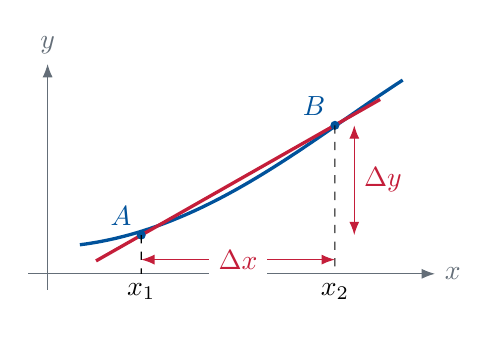
\begin{tikzpicture}[scale=0.82,>=Latex]
    \draw[->,GraphGray] (-0.3,0)--(6.0,0) node[right]{$x$};
    \draw[->,GraphGray] (0,-0.25)--(0,3.25) node[above]{$y$};
    \draw[very thick,JapanBlue] (0.5,0.45) .. controls (2.5,0.7) and (4.1,2.1) .. (5.5,3.0);
    \coordinate (A) at (1.45,0.60);
    \coordinate (B) at (4.45,2.30);
    \draw[very thick,ChinaRed] ($(A)+(-0.7,-0.4)$)--($(B)+(0.7,0.4)$);
    \fill[JapanBlue] (A) circle (2pt) node[above left]{$A$};
    \fill[JapanBlue] (B) circle (2pt) node[above left]{$B$};
    \draw[dashed] (A)--(1.45,0) node[below]{$x_1$};
    \draw[dashed] (B)--(4.45,0) node[below]{$x_2$};
    \draw[<->,ChinaRed] (1.45,0.22)--(4.45,0.22) node[midway,fill=white]{$\Delta x$};
    \draw[<->,ChinaRed] (4.75,0.60)--(4.75,2.30) node[midway,right]{$\Delta y$};
  \end{tikzpicture}
  \end{center}
\end{frame}

% Page 4: the requested limit-definition derivation.
\begin{frame}{微分係数の定義：$y=x^2$}
  \small
  \begin{definition}[Derivative]
    $h$ を $0$ に近づけると、割線の斜率趋近于接线斜率：
    \[
      f'(x)=\frac{\dd y}{\dd x}
      =\lim_{h\to0}\frac{f(x+h)-f(x)}{h}.
    \]
  \end{definition}

  \begin{alertblock}{例：$f(x)=x^2$}
  \scriptsize
  \begin{align*}
    f'(x)
      &=\lim_{h\to0}\frac{(x+h)^2-x^2}{h}\\
      &=\lim_{h\to0}\frac{\bigl[(x+h)-x\bigr]\bigl[(x+h)+x\bigr]}{h}
        &&\text{平方差：$a^2-b^2=(a-b)(a+b)$}\\
      &=\lim_{h\to0}\frac{h(2x+h)}{h}
       =\lim_{h\to0}(2x+h)=\boxed{2x}.
  \end{align*}
  \end{alertblock}
\end{frame}

% Page 5: a clear geometric picture of the same limit.
\begin{frame}{極限のイメージ：割線から接線へ}
  \begin{columns}[T,onlytextwidth]
    \column{0.57\textwidth}
    \begin{center}
    \begin{tikzpicture}[x=1.25cm,y=1.0cm,>=Latex]
      \draw[->,GraphGray] (-0.35,0)--(3.7,0) node[right]{$x$};
      \draw[->,GraphGray] (0,-0.3)--(0,3.2) node[above]{$y$};
      \draw[very thick,JapanBlue,domain=-0.1:3.1,samples=60]
        plot (\x,{0.28*\x*\x}) node[right]{$y=x^2$};
      \coordinate (P) at (1.55,0.673);
      \coordinate (Q) at (2.55,1.821);
      \fill[JapanBlue] (P) circle (2pt) node[below right]{$P(x,x^2)$};
      \fill[ChinaRed] (Q) circle (2pt) node[above left]{$Q(x+h,(x+h)^2)$};
      \draw[thick,ChinaRed] ($(P)+(-0.7,-0.80)$)--($(Q)+(0.65,0.75)$)
        node[right]{割線};
      \draw[thick,JapanBlue,dashed] ($(P)+(-0.85,-0.74)$)--($(P)+(1.30,1.13)$)
        node[above]{接線};
      \draw[<->] (1.55,0.22)--(2.55,0.22) node[midway,fill=white]{$h$};
    \end{tikzpicture}
    \end{center}

    \column{0.40\textwidth}
    \begin{block}{読み方}
      \begin{itemize}
        \item $h\neq0$：两个不同点决定\jp{割線}。
        \item $h\to0$：$Q$ 沿曲线靠近 $P$。
        \item 极限存在时，割线趋近\jp{接線}。
      \end{itemize}
    \end{block}
    \begin{alertblock}{瞬間変化率}
      接线斜率就是函数在该点的\key{瞬时变化率}（instantaneous rate）。
    \end{alertblock}
  \end{columns}
\end{frame}

% Page 6: ordinary derivative formulas.
\begin{frame}{基本的な導関数}
  \scriptsize
  \begin{columns}[T,onlytextwidth]
    \column{0.49\textwidth}
    \begin{block}{代数・指数・対数}
      \renewcommand{\arraystretch}{1.14}
      \begin{tabular}{>{$}l<{$} >{$}l<{$}}
        \toprule
        f(x) & f'(x)\\
        \midrule
        C & 0\\
        x^n & nx^{n-1}\\
        \sqrt{x} & \dfrac{1}{2\sqrt{x}}\\
        \dfrac{1}{x} & -\dfrac{1}{x^2}\\
        e^x & e^x\\
        a^x & a^x\ln a\\
        \ln x & \dfrac{1}{x}\\
        \log_a x & \dfrac{1}{x\ln a}\\
        \bottomrule
      \end{tabular}
    \end{block}

    \column{0.49\textwidth}
    \begin{block}{三角関数（Trigonometric functions）}
      \renewcommand{\arraystretch}{1.15}
      \begin{tabular}{>{$}l<{$} >{$}l<{$}}
        \toprule
        f(x) & f'(x)\\
        \midrule
        \sin x & \cos x\\
        \cos x & -\sin x\\
        \tan x & \dfrac{1}{\cos^2x}\\
        \arcsin x & \dfrac{1}{\sqrt{1-x^2}}\\
        \arccos x & -\dfrac{1}{\sqrt{1-x^2}}\\
        \arctan x & \dfrac{1}{1+x^2}\\
        \bottomrule
      \end{tabular}
    \end{block}

    \begin{alertblock}{注意}
      三角函数求导时，角度必须使用\jp{ラジアン}（radian）。
    \end{alertblock}
  \end{columns}
  \vspace{-0.4em}
  {\tiny 公式整理参考：[Stewart, 2016].}
\end{frame}

% Page 7: sum, difference, and scalar multiple.
\begin{frame}{微分の計算法則 I：和・差・定数倍}
  \begin{columns}[T,onlytextwidth]
    \column{0.48\textwidth}
    \begin{block}{法則}
      \begin{align*}
        \bigl(cf(x)\bigr)' &= c f'(x),\\
        \bigl(f(x)+g(x)\bigr)' &= f'(x)+g'(x),\\
        \bigl(f(x)-g(x)\bigr)' &= f'(x)-g'(x).
      \end{align*}
    \end{block}
    中文理解：每一项可以\key{分别求导}，常数因子保持不变。

    \column{0.49\textwidth}
    \begin{alertblock}{例}
      \[
        y=3x^4-2x^2+5
      \]
      \begin{align*}
        y'
          &=3(4x^3)-2(2x)+0\\
          &=\boxed{12x^3-4x}.
      \end{align*}
    \end{alertblock}
    \begin{block}{セルフチェック}
      常数 $5$ 不随 $x$ 变化，所以其导数为 $0$。
    \end{block}
  \end{columns}
\end{frame}

% Page 8: product and quotient.
\begin{frame}{微分の計算法則 II：積・商}
  \begin{columns}[T,onlytextwidth]
    \column{0.49\textwidth}
    \begin{block}{積の微分（Product Rule）}
      \[
        (fg)'=f'g+fg'
      \]
      \textbf{例：} $y=x^2\sin x$
      \[
        y'=2x\sin x+x^2\cos x.
      \]
      两个函数相乘时，\key{不能}直接写成 $f'g'$。
    \end{block}

    \column{0.49\textwidth}
    \begin{alertblock}{商の微分（Quotient Rule）}
      \[
        \left(\frac{f}{g}\right)'
        =\frac{f'g-fg'}{g^2},\qquad g\neq0
      \]
      \textbf{例：} $y=\dfrac{x+1}{x-1}$
      \[
        y'=\frac{(x-1)-(x+1)}{(x-1)^2}
        =\boxed{-\frac{2}{(x-1)^2}}.
      \]
    \end{alertblock}
  \end{columns}

  \centering
  \vspace{0.4em}
  \jp{记忆：積是“前导后不导＋前不导后导”；商的分母最后平方。}
\end{frame}

% Page 9: physics connection, closing the derivative section.
\begin{frame}{物理とのつながり：位置・速度・加速度}
  \begin{columns}[T,onlytextwidth]
    \column{0.54\textwidth}
    \begin{block}{時間による微分}
      \[
        \text{位置 }x(t)
        \xrightarrow{\;\dd/\dd t\;}
        \text{速度 }v(t)
        \xrightarrow{\;\dd/\dd t\;}
        \text{加速度 }a(t)
      \]
      \[
        v(t)=\frac{\dd x}{\dd t},\qquad
        a(t)=\frac{\dd v}{\dd t}=\frac{\dd^2x}{\dd t^2}.
      \]
    \end{block}
    导数描述物理量\key{此刻怎样变化}，是运动学的共同语言。

    \column{0.43\textwidth}
    \begin{alertblock}{例}
      若
      \[
        x(t)=2t^3-3t^2+4,
      \]
      则
      \[
        v(t)=6t^2-6t,
      \]
      \[
        a(t)=12t-6.
      \]
    \end{alertblock}
    \begin{center}
      \key{微分部分終了}
    \end{center}
  \end{columns}
\end{frame}

\section{ベクトル}

% Page 10: vector introduction.
\begin{frame}{ベクトルとは何か}
  \begin{columns}[T,onlytextwidth]
    \column{0.52\textwidth}
    \begin{block}{スカラーとベクトル}
      \begin{itemize}
        \item \jp{スカラー量}（scalar）：只有大小。例：质量、时间、温度。
        \item \jp{ベクトル量}（vector）：同时具有大小和方向。例：位移、速度、加速度、力。
      \end{itemize}
    \end{block}
    \[
      \vec A=(A_x,A_y),\qquad
      |\vec A|=\sqrt{A_x^2+A_y^2}.
    \]

    \column{0.45\textwidth}
    \begin{center}
    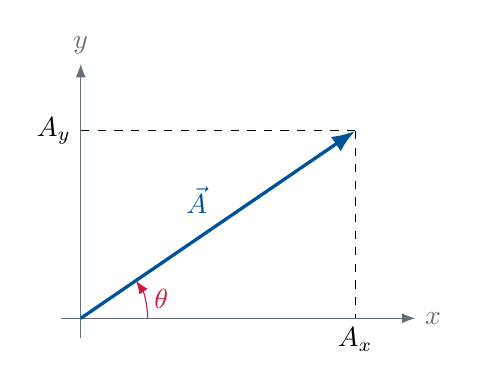
\begin{tikzpicture}[x=0.85cm,y=0.85cm,>=Latex]
      \draw[->,GraphGray] (-0.3,0)--(5.0,0) node[right]{$x$};
      \draw[->,GraphGray] (0,-0.3)--(0,3.8) node[above]{$y$};
      \draw[->,very thick,JapanBlue] (0,0)--(4.1,2.8)
        node[midway,above left]{$\vec A$};
      \draw[dashed] (4.1,2.8)--(4.1,0) node[below]{$A_x$};
      \draw[dashed] (4.1,2.8)--(0,2.8) node[left]{$A_y$};
      \draw[->,ChinaRed] (1.0,0) arc[start angle=0,end angle=34.3,radius=1.0]
        node[midway,right]{$\theta$};
    \end{tikzpicture}
    \end{center}
    \begin{alertblock}{符号}
      箭头 $\vec A$ 表示矢量；$|\vec A|$ 表示它的大小。
    \end{alertblock}
  \end{columns}
\end{frame}

% Page 11: decomposition.
\begin{frame}{ベクトルの成分分解（Decomposition）}
  \begin{columns}[T,onlytextwidth]
    \column{0.52\textwidth}
    \begin{center}
    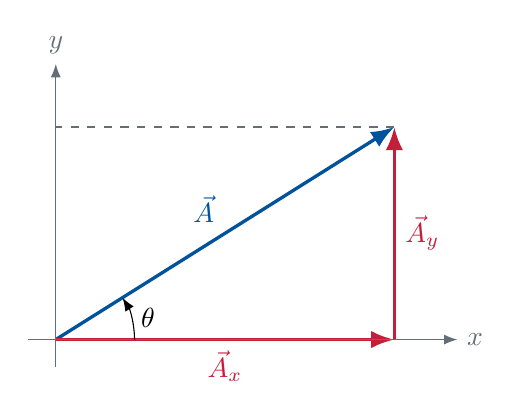
\begin{tikzpicture}[x=1.0cm,y=1.0cm,>=Latex]
      \coordinate (O) at (0,0);
      \coordinate (P) at (4.3,2.7);
      \draw[->,very thick,JapanBlue] (O)--(P) node[midway,above left]{$\vec A$};
      \draw[->,very thick,ChinaRed] (O)--(4.3,0) node[midway,below]{$\vec A_x$};
      \draw[->,very thick,ChinaRed] (4.3,0)--(P) node[midway,right]{$\vec A_y$};
      \draw[dashed,GraphGray] (P)--(0,2.7);
      \draw[->,GraphGray] (-0.35,0)--(5.1,0) node[right]{$x$};
      \draw[->,GraphGray] (0,-0.35)--(0,3.5) node[above]{$y$};
      \draw[->] (1.0,0) arc[start angle=0,end angle=32.1,radius=1.0]
        node[midway,right]{$\theta$};
    \end{tikzpicture}
    \end{center}

    \column{0.45\textwidth}
    \begin{block}{直角座標で分ける}
      \[
        A_x=A\cos\theta,
        \qquad
        A_y=A\sin\theta.
      \]
      \[
        A=\sqrt{A_x^2+A_y^2},
        \qquad
        \tan\theta=\frac{A_y}{A_x}.
      \]
    \end{block}
    \begin{alertblock}{物理例}
      斜面问题中，把重力分解为平行和垂直于斜面的两个分量。
    \end{alertblock}
  \end{columns}
\end{frame}

% Page 12: composition and arithmetic.
\begin{frame}{ベクトルの合成・差・実数倍}
  \begin{columns}[T,onlytextwidth]
    \column{0.53\textwidth}
    \begin{center}
    \begin{tikzpicture}[x=0.9cm,y=0.9cm,>=Latex]
      \coordinate (O) at (0,0);
      \coordinate (A) at (3.4,0.8);
      \coordinate (B) at (1.3,2.5);
      \coordinate (R) at ($(A)+(B)$);
      \draw[->,very thick,JapanBlue] (O)--(A) node[midway,below]{$\vec A$};
      \draw[->,very thick,ChinaRed] (O)--(B) node[midway,left]{$\vec B$};
      \draw[dashed,JapanBlue] (B)--(R);
      \draw[dashed,ChinaRed] (A)--(R);
      \draw[->,ultra thick,black] (O)--(R) node[midway,above left]{$\vec R$};
      \node[below] at (2.3,-0.4) {平行四辺形法};
    \end{tikzpicture}
    \end{center}

    \column{0.44\textwidth}
    \begin{block}{成分で計算}
      \begin{align*}
        \vec A+\vec B
          &=(A_x+B_x,\ A_y+B_y),\\
        \vec A-\vec B
          &=(A_x-B_x,\ A_y-B_y),\\
        k\vec A&=(kA_x,\ kA_y).
      \end{align*}
    \end{block}
    \begin{alertblock}{合成（Composition）}
      首尾相接法和平行四边形法得到同一个合矢量：
      \[
        \vec R=\vec A+\vec B.
      \]
    \end{alertblock}
  \end{columns}
\end{frame}

% Page 13: dot product.
\begin{frame}{内積（Dot Product / Scalar Product）}
  \begin{columns}[T,onlytextwidth]
    \column{0.52\textwidth}
    \begin{block}{定義}
      \[
        \vec A\cdot\vec B
        =|\vec A||\vec B|\cos\theta
        =A_xB_x+A_yB_y.
      \]
      计算结果是一个\key{スカラー}（scalar）。
    \end{block}
    \begin{itemize}
      \item $\vec A\cdot\vec B>0$：夹角为锐角。
      \item $\vec A\cdot\vec B=0$：两矢量垂直。
      \item $\vec A\cdot\vec B<0$：夹角为钝角。
    \end{itemize}

    \column{0.45\textwidth}
    \begin{center}
    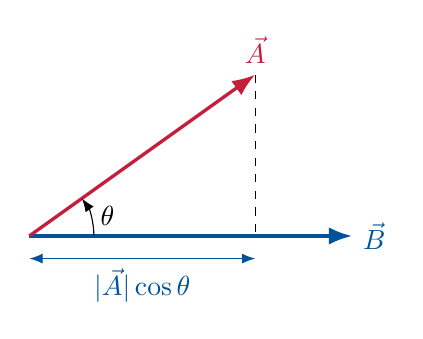
\begin{tikzpicture}[x=0.82cm,y=0.82cm,>=Latex]
      \draw[->,very thick,JapanBlue] (0,0)--(5.0,0) node[right]{$\vec B$};
      \draw[->,very thick,ChinaRed] (0,0)--(3.5,2.5) node[above]{$\vec A$};
      \draw[dashed] (3.5,2.5)--(3.5,0);
      \draw[<->,JapanBlue] (0,-0.35)--(3.5,-0.35)
        node[midway,below]{$|\vec A|\cos\theta$};
      \draw[->] (1.0,0) arc[start angle=0,end angle=35.5,radius=1.0]
        node[midway,right]{$\theta$};
    \end{tikzpicture}
    \end{center}
    \begin{alertblock}{物理例：仕事}
      \[
        W=\vec F\cdot\vec s=Fs\cos\theta.
      \]
      只有力在位移方向上的分量做功。
    \end{alertblock}
  \end{columns}
  \vspace{-0.2em}
  {\tiny ベクトルと仕事の整理参考：[Ling et al., 2022].}
\end{frame}

% Page 14: cross product as an extension.
\begin{frame}{外積（Cross Product）— 発展内容}
  \begin{columns}[T,onlytextwidth]
    \column{0.52\textwidth}
    \begin{block}{大きさと向き}
      \[
        |\vec A\times\vec B|
        =|\vec A||\vec B|\sin\theta.
      \]
      结果是一个垂直于 $\vec A$、$\vec B$ 所在平面的\key{ベクトル}。
      方向由\jp{右手の法則}（right-hand rule）决定。
    \end{block}
    \begin{itemize}
      \item 平行：$\vec A\times\vec B=\vec0$
      \item 垂直：外积大小最大
      \item 顺序反转：$\vec B\times\vec A=-(\vec A\times\vec B)$
    \end{itemize}

    \column{0.45\textwidth}
    \begin{center}
    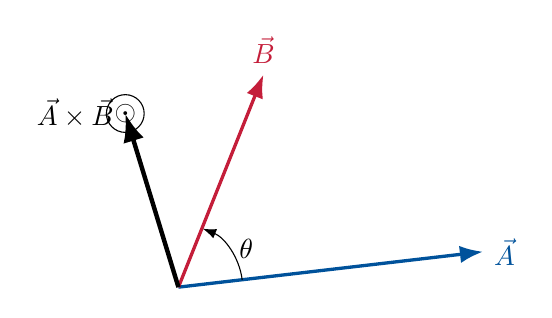
\begin{tikzpicture}[x=0.9cm,y=0.9cm,>=Latex]
      \draw[->,very thick,JapanBlue] (0,0)--(4.3,0.5) node[right]{$\vec A$};
      \draw[->,very thick,ChinaRed] (0,0)--(1.2,3.0) node[above]{$\vec B$};
      \draw[->,ultra thick,black] (0,0)--(-0.75,2.45)
        node[left]{$\vec A\times\vec B$};
      \draw[->] (0.9,0.10) arc[start angle=7,end angle=68,radius=0.9]
        node[midway,right]{$\theta$};
      \node[draw,circle,inner sep=1.2pt] at (-0.75,2.45) {$\odot$};
    \end{tikzpicture}
    \end{center}
    \begin{alertblock}{物理例：力のモーメント}
      \[
        \vec\tau=\vec r\times\vec F,
        \qquad |\tau|=rF\sin\theta.
      \]
    \end{alertblock}
  \end{columns}
\end{frame}

\section{練習と参考文献}

% Page 15: derivative exercises.
\begin{frame}{練習問題 I：微分}
  \begin{enumerate}
    \item 定义式を用いて，$f(x)=x^2$ 在 $x=2$ 处的导数值を求めよ。
    \vspace{0.45em}
    \item 次の導関数を求めよ。
      \[
        \text{(a) }y=3x^4-2x^2+5,
        \qquad
        \text{(b) }y=x^2\sin x,
        \qquad
        \text{(c) }y=\frac{x+1}{x-1}.
      \]
    \item 物体的位置为 $x(t)=2t^3-3t^2+4$。求 $v(t)$、$a(t)$，以及 $t=1$ 时的速度。
  \end{enumerate}

  \begin{alertblock}{ヒント}
    (1) 先写 $f(2+h)-f(2)$；(2b) 用\jp{積の微分}；(2c) 用\jp{商の微分}。
  \end{alertblock}
\end{frame}

% Page 16: vector exercises and compact answers.
\begin{frame}{練習問題 II：ベクトル}
  \small
  \begin{columns}[T,onlytextwidth]
    \column{0.56\textwidth}
    \begin{enumerate}
      \item $|\vec A|=10$、$\theta=30^\circ$。$A_x,A_y$ を求めよ。
      \item $\vec A=(3,4)$、$\vec B=(-1,2)$。次を求めよ：
        \[
          \vec A+\vec B,\quad \vec A-\vec B,\quad
          |\vec A|,\quad \vec A\cdot\vec B.
        \]
      \item $F=20\,\mathrm{N}$ の力が変位方向と $60^\circ$ をなし、物体が $5\,\mathrm{m}$ 移動した。仕事 $W$ を求めよ。
    \end{enumerate}

    \column{0.41\textwidth}
    \begin{alertblock}{解答}
      \begin{align*}
        1.&\quad (A_x,A_y)=(5\sqrt3,5),\\
        2.&\quad \vec A+\vec B=(2,6),\\
          &\quad \vec A-\vec B=(4,2),\\
          &\quad |\vec A|=5,\quad \vec A\cdot\vec B=5,\\
        3.&\quad W=20\times5\times\cos60^\circ\\
          &\quad\;=50\,\mathrm{J}.
      \end{align*}
    \end{alertblock}
  \end{columns}
\end{frame}

% Page 17: reader-friendly references.
\begin{frame}{参考文献}
  \small
  \begin{columns}[T,onlytextwidth]
    \column{0.48\textwidth}
    \begin{block}{1\quad EJU 公式資料}
      \textbf{日本学生支援機構（JASSO）}\par
      \vspace{0.25em}
      2026年度 日本留学試験\par
      \jp{物理シラバス}\par
      \vspace{0.35em}
      {\scriptsize
      \href{https://www.jasso.go.jp/ryugaku/eju/examinee/syllabus/science_phy.html}
      {\color{JapanBlue}\underline{JASSO 公式ページを開く}}}
    \end{block}

    \begin{alertblock}{2\quad 微分・数学}
      \textbf{James Stewart}\par
      \emph{Calculus: Early Transcendentals}\par
      8th ed., Cengage Learning, 2016.
    \end{alertblock}

    \column{0.48\textwidth}
    \begin{block}{3\quad ベクトル・力学}
      \textbf{S. J. Ling, W. Moebs, J. Sanny}\par
      \emph{University Physics, Volume 1}\par
      OpenStax, Rice University, 2022.\par
      \vspace{0.35em}
      {\scriptsize
      \href{https://openstax.org/details/books/university-physics-volume-1}
      {\color{JapanBlue}\underline{OpenStax で読む}}}
    \end{block}

    \begin{alertblock}{4\quad 発展参考}
      \textbf{R. A. Serway, J. W. Jewett}\par
      \emph{Physics for Scientists and Engineers}\par
      10th ed., Cengage Learning, 2018.
    \end{alertblock}
  \end{columns}

  \vfill
  \centering
  {\footnotesize 本资料以日文物理术语为主，中文解释帮助理解，英文术语用于补充。}
\end{frame}

\end{document}
